\documentclass{standalone}
\author{Quinten Bruynseraede}
\usepackage{tikz}
\usetikzlibrary{shapes}
\title{Tikz grafen}
\begin{document}\pagestyle{empty}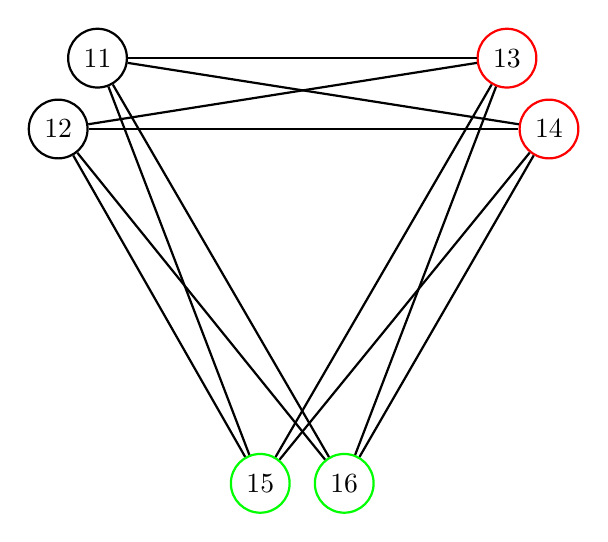
\begin{tikzpicture}\node[shape=circle,draw=green,align=center,line width=0.8pt] (0) at (5.7,8.566666666666666) {15};
\node[shape=circle,draw=green,align=center,line width=0.8pt] (1) at (6.766666666666667,8.566666666666666) {16};
\node[shape=circle,draw=red,align=center,line width=0.8pt] (2) at (8.833333333333334,13.966666666666667) {13};
\node[shape=circle,draw=red,align=center,line width=0.8pt] (3) at (9.366666666666667,13.066666666666666) {14};
\node[shape=circle,draw=black,align=center,line width=0.8pt] (4) at (3.6333333333333333,13.966666666666667) {11};
\node[shape=circle,draw=black,align=center,line width=0.8pt] (5) at (3.1333333333333333,13.066666666666666) {12};

\path [-,draw=black,line width=0.8pt] (4) edge node {} (2);
\path [-,draw=black,line width=0.8pt] (4) edge node {} (3);
\path [-,draw=black,line width=0.8pt] (4) edge node {} (1);
\path [-,draw=black,line width=0.8pt] (4) edge node {} (0);
\path [-,draw=black,line width=0.8pt] (5) edge node {} (2);
\path [-,draw=black,line width=0.8pt] (5) edge node {} (3);
\path [-,draw=black,line width=0.8pt] (5) edge node {} (1);
\path [-,draw=black,line width=0.8pt] (5) edge node {} (0);
\path [-,draw=black,line width=0.8pt] (2) edge node {} (0);
\path [-,draw=black,line width=0.8pt] (2) edge node {} (1);
\path [-,draw=black,line width=0.8pt] (3) edge node {} (1);
\path [-,draw=black,line width=0.8pt] (3) edge node {} (0);
\end{tikzpicture}
\end{document}